\subsection{An Introduction to Pointers}
The textbook definition of a pointer is \textit{The pointer in C language is a variable which stores the address of another variable.} This variable can be of type int, char, array, function, or any other pointer. The size of the pointer depends on the architecture. 

\subsubsection{Pointer Notation}
Consider the declaration,\quad \textbf{int i = 3;}\\
This declaration tells the C compiler to:
\begin{enumerate}
    \item Reserve space in memory to hold the integer value.
    \item Associate the name i with this memory location.
    \item Store the value 3 at this location.
\end{enumerate}
We may represent i’s location in memory by the following memory map.
\begin{figure}[H]
    \begin{center}
        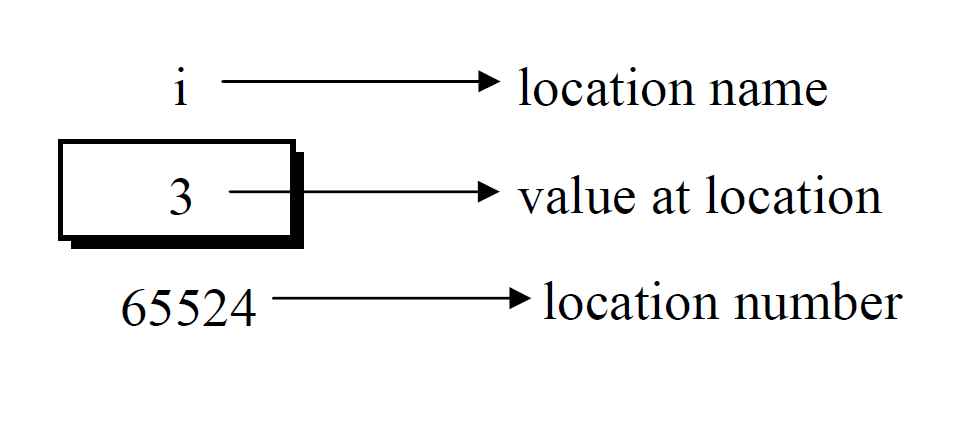
\includegraphics[width=\textwidth]{images/pointer.png}
        \caption{Variable memory map}
        \label{pointer}
    \end{center}
\end{figure}

We see that the computer has selected memory location 65524 as the place to store the value 3. \textbf{i’s address in memory is a number.}

\paragraph{Operator \&} "\&" is used in  C as an "address of" operator. The expression "\&i" returns the address of the variable i, which in this case happens to be 65524. We have been using the "\&" operator all the time in the scanf() statement.

\paragraph{Operator *} Pointer operator "*" is called as the "value at address" operator. It gives the value stored at a particular address. The "value at address" operator is also called "indirection" operator

Note that printing the value of "*(\&i)" is same as printing the value of i.

The expression \&i gives the address of the variable i. This address can be collected in a variable, by saying,
j = \&i ;

But remember that j is not an ordinary variable like any other integer variable. It is a variable that contains the address of other variable (i in this case). Since j is a variable the compiler must provide it space in the memory. 


\paragraph{Pointer declaration}
int *j;\\
This declaration tells the compiler that j will be used to store the address of an integer value. In other words, j points to an integer. 

Here is a program that demonstrates the relationships we have been discussing.

\begin{lstlisting}[style=CStyle]
main( )
{
    int i = 3 ;
    int *j ;

    j = &i ;
    printf ( "\nAddress of i = %u", &i ) ;
    printf ( "\nAddress of i = %u", j ) ;
    printf ( "\nAddress of j = %u", &j ) ;
    printf ( "\nValue of j = %u", j ) ;
    printf ( "\nValue of i = %d", i ) ;
    printf ( "\nValue of i = %d", *( &i ) ) ;
    printf ( "\nValue of i = %d", *j ) ;
}
\end{lstlisting}
The output of the above program would be:
\begin{lstlisting}[style=CStyle]
    Address of i = 65524
    Address of i = 65524
    Address of j = 65522
    Value of j = 65524
    Value of i = 3
    Value of i = 3
    Value of i = 3
\end{lstlisting}

\textbf{\textit{Note: Remember that, addresses (location numbers) are always going to be whole numbers, therefore pointers always contain whole numbers.}}